\section{Przebieg procesu uczenia}
\label{sec:wyniki-przebieg-uczenia}

W~tej sekcji przedstawiono, jak kształtował się przebieg treningu.
W~tym celu wykorzystano okresowe pomiary walidacyjne
wykonywane zgodnie z~procedurą opisaną w~
rozdziale~\ref{chap:eksperymenty}. Każdy punkt krzywej odpowiada
ewaluacji aktualnej polityki na 2\,000 wspólnych rozdań
walidacyjnych.

Wyniki walidacyjne są traktowane jako opis dynamiki procesu uczenia,
a~nie jako zamiennik końcowej ewaluacji na 100\,000 niezależnych
rozdań. Mniejsza liczba rozdań w~pojedynczym punkcie powoduje większą
zmienność oszacowanego EV, jednak wspólny harmonogram walidacyjny
umożliwia bezpośrednie porównywanie kolejnych punktów kontrolnych.

Na rysunku~\ref{fig:dqn-learning-curves} przedstawiono przebieg
treningu czterech konfiguracji DQN. Na osi poziomej znajduje się
liczba epizodów treningowych, a~na osi pionowej walidacyjne EV.
Linie przedstawiają średnie z~pięciu ziaren, a~pasma jedno
odchylenie standardowe między przebiegami treningowymi. Widać na
nim, że warianty FEATURES przez cały trening utrzymują się wyraźnie
powyżej wariantów RAW, a~odstęp między krzywymi nie zmniejsza się
znacząco w~czasie trwania treningu.

\begin{figure}[htbp]
    \centering
    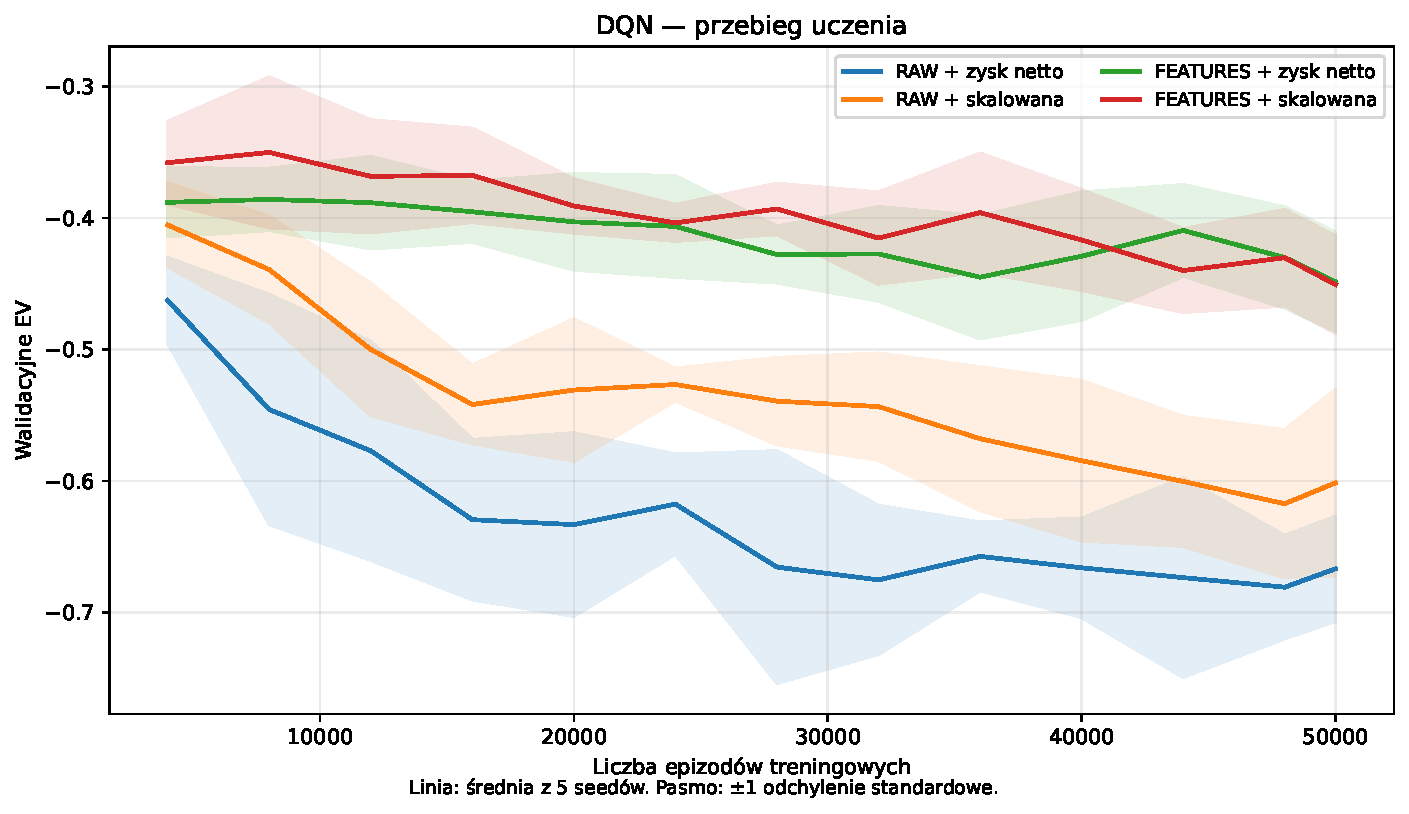
\includegraphics[
        width=\textwidth
    ]{../experiments/results/final_analysis/04_dqn_learning_curves.pdf}
    \caption{Przebieg uczenia czterech konfiguracji DQN}
    \label{fig:dqn-learning-curves}
\end{figure}

Już w~trakcie treningu widoczna jest różnica pomiędzy
reprezentacjami RAW i~FEATURES. Oba warianty wykorzystujące FEATURES
utrzymują przeciętnie wyższe EV niż odpowiadające im warianty RAW.
Jest to zgodne z~wynikami końcowej ewaluacji przedstawionymi
w~sekcji~\ref{sec:wyniki-reprezentacja-stanu}.

Jednocześnie krzywe nie wykazują monotonicznego wzrostu jakości
polityki. Po okresach poprawy występują lokalne spadki wartości EV. Oznacza to, że
dalsze wykonywanie aktualizacji sieci
nie gwarantuje poprawy strategii na każdym kolejnym punkcie kontrolnym.
Zjawisko to występuje również dla konfiguracji FEATURES.

Analogiczne wyniki dla REINFORCE przedstawiono na
rysunku~\ref{fig:reinforce-learning-curves}, z~tymi samymi osiami i~tym samym
sposobem uśredniania. Krzywe REINFORCE są znacznie mniej gładkie niż
dla DQN, a~pasma odchylenia standardowego są szersze i~w~wielu
punktach przecinają się nawzajem, co wskazuje, że w~tym samym momencie
treningu różne konfiguracje mogą osiągać porównywalną jakość polityki.

\begin{figure}[htbp]
    \centering
    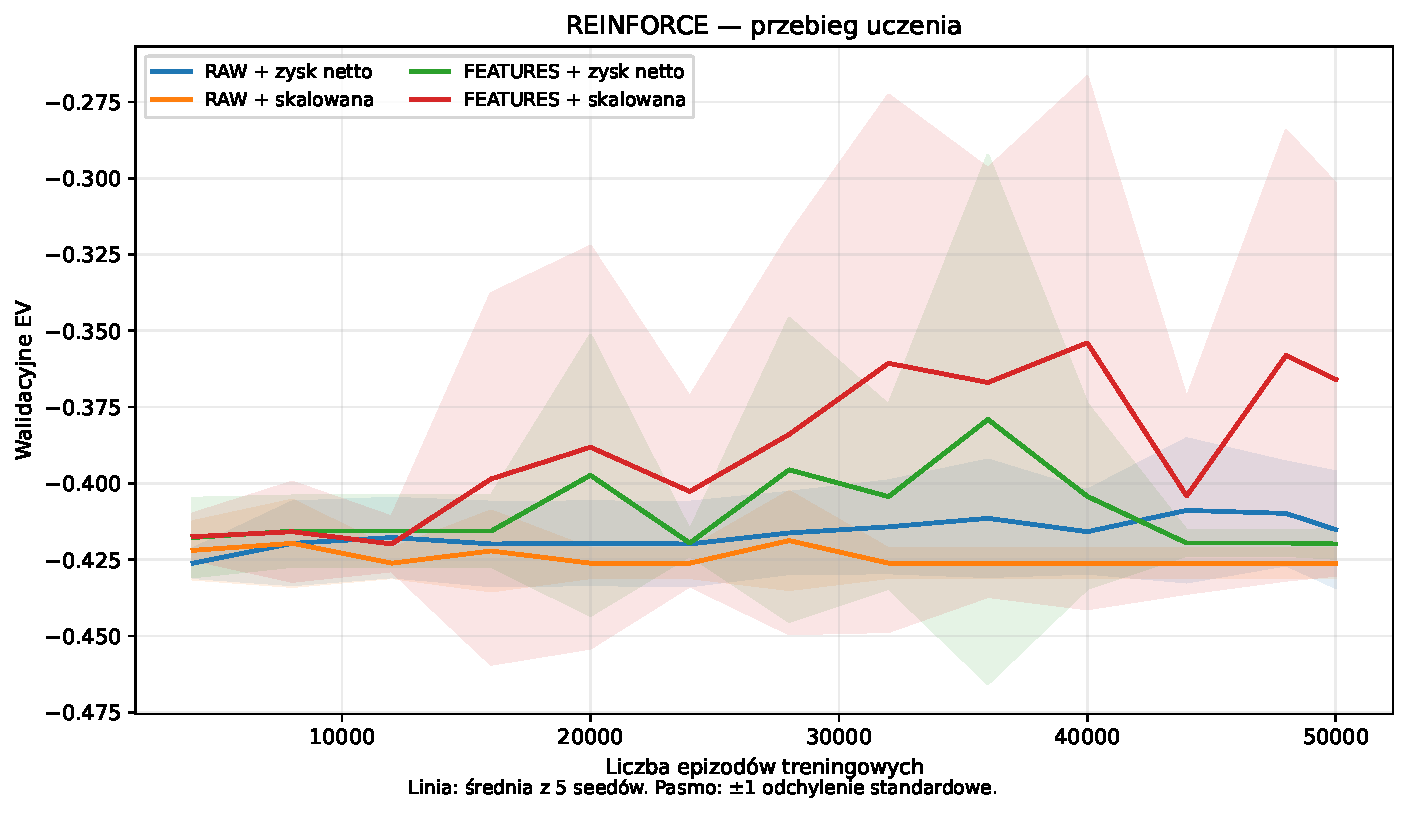
\includegraphics[
        width=\textwidth
    ]{../experiments/results/final_analysis/05_reinforce_learning_curves.pdf}
    \caption{Przebieg uczenia czterech konfiguracji REINFORCE}
    \label{fig:reinforce-learning-curves}
\end{figure}

Konfiguracja FEATURES ze skalowaną funkcją nagrody osiągnęła najwyższe średnie EV spośród
konfiguracji REINFORCE w~końcowej ewaluacji, ale jednocześnie
charakteryzowała się największym odchyleniem standardowym między
ziarnami. Krzywe walidacyjne pokazują, że zróżnicowanie to powstaje już
podczas procesu uczenia i~nie jest wyłącznie efektem końcowej
ewaluacji.
